% !TEX TS-program = xelatex
\documentclass[11pt]{article}
\usepackage{lindrew}
\usepackage{tikz}
\usepackage{pgfplots}
\usepackage{fontspec}
\pgfplotsset{compat=1.18}
\title{Math 4580: Abstract Algebra I}
\usepackage{hyperref}
\hypersetup{
    colorlinks=true,
    linkcolor=red,
    filecolor=red,
    urlcolor=red,
    citecolor=red
}
\author{Lecturer: \textbf{Professor Michael Lipnowski}\\Notes by: Farhan Sadeek}
\date{Spring 2025}

\begin{document}

\maketitle
%%%%%%%%%%%%%%%%%%%%%%%%%%%%

\section{January 6, 2025}
We didn't have any, but Dr.\ Lipnowski did post a module on
\href{https://carmen.osu.edu}{{\texttt{carmen}}} about the syllabus and the
course. This semester we will be covering the first few chapters of the book
\textit{Abstract Algebra: Theory and Applications} by Thomas Judson. \\

\begin{definition}
    \vocab{Set}: A collection of distinct objects, considered as an object in its own right.\\
    \vocab{Axioms}: A collection of objects \( \mathrm{S} \) with assumed structural rules is defined by axioms.\\
    \vocab{Statement}: In logic or mathematics, an assertion that is either true or false.\\
    \vocab{Hypothesis and Conclusion}: In the statement ``If P, then Q'', P is the hypothesis and Q is the conclusion.\\
    \vocab{Mathematical Proof}: A logical argument that verifies the truth of a statement.\\
    \vocab{Proposition}: A statement that can be proven true.\\
    \vocab{Theorem}: A proposition of significant importance.\\
    \vocab{Lemma}: A supporting proposition used to prove a theorem or another proposition.\\
    \vocab{Corollary}: A proposition that follows directly from a theorem or proposition with minimal additional proof.
\end{definition}

\section{January 8, 2025}
Professor Lipnowski discussed Sam Lloyd's 15 puzzle. Each lecture will include
a mystery digit, contributing up to 5\% bonus to the final grade based on
correct guesses.

Certain course expectations:
\begin{itemize}
    \item All assignments (one every two weeks) and exams (one midterm and one final
          exam) will be take-home.
    \item All the problems from the course textbook.
    \item Collaboration is encouraged, but the work should be your own.
    \item For the exams, we are not supposed to talk to other friends.
\end{itemize}

\subsection{Functions}
\begin{definition}
    Let $A$ and $B$ be sets. A function $f: A \to B$ assigns exactly one output $f(a) \in B$ to every input $a \in A$.
\end{definition}
\begin{itemize}
    \item The set $A$ is called the \textbf{domain} of $f$.
    \item The set $B$ is called the \textbf{codomain} of $f$.
\end{itemize}

\begin{fact}The domain $A$, codomain $B$, and the assignment of outputs $f(a)$ to every input $a \in A$ are all part of the data defining a function. Just writing a formula like $f(x) = e^x$ does not determine a function, as the domain and codomain are not specified.
\end{fact}
For example:
\begin{itemize}
    \item $f: \mathbb{R} \to \mathbb{R}, f(x) = e^x$.
    \item $f: \mathbb{Q} \to \mathbb{Q}, f(x) = e^x$.
\end{itemize}
Although these functions use the same formula, their meanings are completely different because their domains and codomains differ.

\subsection{Graphs}
A function $f: A \to B$ is often identified with its \textbf{graph} in $A
    \times B$:
\[ \text{graph}(f) = \{(a, b) \in A \times B : b = f(a)\}. \]

\begin{lemma}
    Let $f: A \to B$ be a function. Its graph, $\text{graph}(f)$, passes the \textbf{vertical line test}: For every $a \in A$, $V_a := \{(a, b) \in A \times B : b \in B\}$ intersects $\text{graph}(f)$ in exactly one element.
\end{lemma}
\begin{center}
    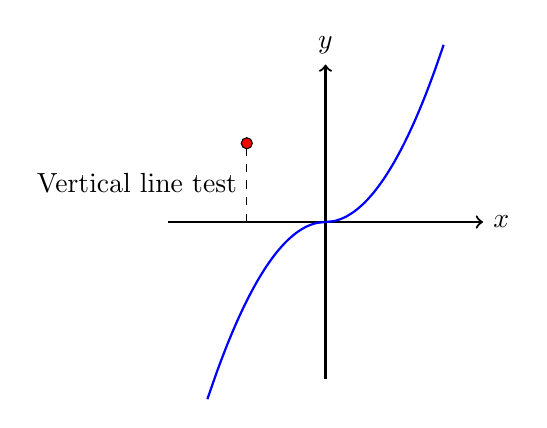
\begin{tikzpicture}
        \draw[thick,->] (-2,0) -- (2,0) node[right] {$x$};
        \draw[thick,->] (0,-2) -- (0,2) node[above] {$y$};
        \draw[domain=-1.5:1.5,smooth,variable=\x,blue,thick] plot ({\x},{\x^2});
        \draw[dashed] (-1,0) -- (-1,1) node[midway,left] {Vertical line test};
        \draw[fill=red] (-1,1) circle (2pt);
    \end{tikzpicture}
\end{center}

\begin{proposition}
    Let $G \subseteq A \times B$ be any subset passing the vertical line test, i.e., for all $a \in A$, $V_a \cap G$ consists of exactly one element. Then $G = \text{graph}(f)$ for a unique function $f: A \to B$.
\end{proposition}
\begin{proof}
    If $G = \{(a, b) \mid b \in B\}$ satisfies the vertical line test, define $f: A \to B$ by $f(a) = b$. Then $G = \text{graph}(f)$.
\end{proof}

\begin{definition}
    A subset $R \subseteq A \times B$ is called a \textbf{relation}. The vertical line test distinguishes graphs of functions from more general relations.
\end{definition}
\subsection{Examples}
\begin{itemize}
    \item Let $S = \{(x, y) \in \mathbb{R}^2 : x^2 + y^2 = 1\}$ (the unit circle). This
          is a relation but not the graph of a function because it fails the vertical
          line test: The vertical line $x = 0$ intersects the circle at two points.
    \item Visual depiction of a unit circle:
          \begin{center}
              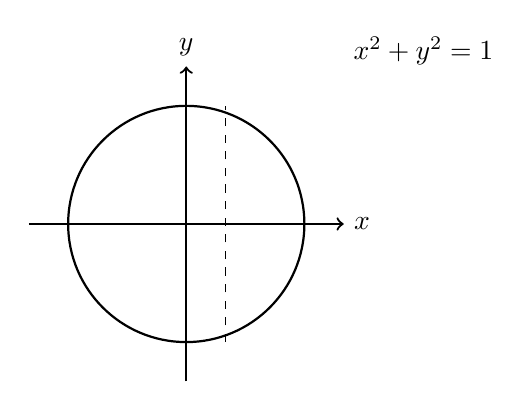
\begin{tikzpicture}
                  \draw[thick,->] (-2,0) -- (2,0) node[right] {$x$};
                  \draw[thick,->] (0,-2) -- (0,2) node[above] {$y$};
                  \draw[thick] (0,0) circle (1.5);
                  \node[below right] at (2,2.5) {$x^2 + y^2 = 1$};
                  \draw[dashed] (0.5,-1.5) -- (0.5,1.5);
              \end{tikzpicture}
          \end{center}
    \item Let $A = \{1, 2, 3\}$, $B = \{4, 5\}$. The number of functions from $A$ to $B$
          is $2^3 = 8$, corresponding to the $8$ associated graphs in $A \times B$.
    \item The number of relations from $A$ to $B$ is $2^{ |a| \cdot |b|} = 2^{3 \cdot 2}
              = 64$, containing the $8$ graphs of functions from $A$ to $B$.
\end{itemize}

\begin{fact}
    The notion of relation is much more permissive than the notion of functions.
\end{fact}

\subsection{Visualizing Functions as Directed Edges}
A function $f: A \to B$ can be visualized as a collection of directed edges
$(a, f(a)) \in A \times B$. Each element of $A$ has exactly one outgoing edge
in the graph.

\begin{center}
    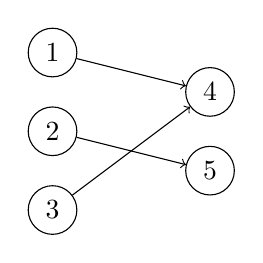
\begin{tikzpicture}
        \node[circle,draw] (A1) at (0,1) {$1$};
        \node[circle,draw] (A2) at (0,0) {$2$};
        \node[circle,draw] (A3) at (0,-1) {$3$};
        \node[circle,draw] (B1) at (2,0.5) {$4$};
        \node[circle,draw] (B2) at (2,-0.5) {$5$};
        \draw[->] (A1) -- (B1);
        \draw[->] (A2) -- (B2);
        \draw[->] (A3) -- (B1);
    \end{tikzpicture}
\end{center}
\section{January 10, 2025}
\subsection{Injection and Surjection}

Let $f : A \to B$ be a function.

\begin{definition}[Injectivity (One-to-One)]

    $f$ is injective (one-to-one) if:
    \[
        \forall x, y \in A, \, f(x) = f(y) \implies x = y
    \]
    Equivalently:
    \[
        x \neq y \implies f(x) \neq f(y)
    \]\end{definition}

\begin{fact} Distinct inputs have distinct outputs.
\end{fact}

\begin{definition}[Surjectivity (Onto)]

    $f$ is surjective (onto) if:
    \[
        \forall b \in B, \, \exists a \in A \text{ such that } f(a) = b.
    \]

\end{definition}

\begin{fact}
    Every $b \in B$ is an output of something through $f$.''

\end{fact}

\begin{example}
    Here are a few examples of injectivity and surjectivity:
    \begin{itemize}

        \item Let $A = \{1, 2, 3\}$ and $B = \{4, 5\}$ and $f: A \to B$ with $f(1), f(2),
                  f(3)$ as elements of $B$. If $B$ has only two elements, at least two of $f(1),
                  f(2), f(3)$ must coincide (e.g., $f(1) = f(2)$). Thus, $f$ is not injective.
        \item Let $A = \{1, 2, 3\}$ and $B = \{4, 5, 6, 7\}$ and $f : A \to B$ where:
              \[
                  f(1) = 4, \, f(2) = 7, \, f(3) = 5.
              \]
              Distinct inputs have distinct outputs, so $f$ is injective.
        \item Let $A = \{1, 2, 3\}$ and $B = \{4, 5, 6, 7\}$ and $f : A \to B$ where:
              \[
                  f(1) = 4, \, f(2) = 4, \, f(3) = 6.
              \]
              Here, $A = \{1, 2, 3\}$ and $B = \{4, 5, 6, 7\}$ and $f(1) = f(2)$ but $1 \neq
                  2$, so $f$ is not injective.
        \item Let $f : A \to B$ where $B$ has size 4 and $f(1), f(2), f(3)$ are distinct
              elements of $B$. If $B \setminus \{f(1), f(2), f(3)\}$ is non-empty, then $b
                  \neq f(a)$ for all \(a \in A\), implying \(f\) is non surjective.
        \item Let $A = \{1, 2, 3\}$ and $B = \{4, 5\}$ and $f: A \to B$ with $f(1) = 4, f(2)
                  = 5, f(3) = 4$. $f$ is surjective.
        \item Let $A = \{1, 2, 3\}$ and $B = \{4, 5\}$ and $f: A \to B$ with $f(1) = 4, f(2)
                  = 4, f(3) = 4$. $f$ is not surjective.
    \end{itemize}
\end{example}

\subsection{Bijection and Range}
\begin{definition} [Bijectivity]

    $f$ is bijective if $f$ is both injective and surjective.
\end{definition}
\begin{definition}

    Let $f : A \to B$ be a function. The \textit{range} of $f$ is the subset of $B$
    defined as:
    \[
        \text{range}(f) := \{ b \in B \mid b = f(a) \text{ for some } a \in A \}.
    \]
    Thus, $f : A \to B$ is surjective \(\Longleftrightarrow\) $\text{range}(f) =
        B$.
\end{definition}

\begin{itemize}
    \item Let $A = \{1, 2, 3\}$ and $B = \{4, 5, 6\}$ and $f : A \to B$ where:
          \[
              f(1) = 6, \, f(2) = 5, \, f(3) = 4.
          \]
          $f$ is a bijection.
    \item Let $A = \{1, 2, 3\}$ and $B = \{4, 5, 6, 7\}$ and $f : A \to B$ where:
          \[
              f(1) = 4, \, f(2) = 4, \, f(3) = 56
          \]
          $f$ is neither injective nor surjective.

\end{itemize}
\begin{question*}
    Let $A$ and $B$ be finite sets of the same size. Prove that the following are
    equivalent:
    \begin{enumerate}
        \item $f : A \to B$ is injective.
        \item $f : A \to B$ is bijective.
        \item $f : A \to B$ is surjective.
    \end{enumerate}
    Demonstrate that (1), (2), and (3) are not necessarily equivalent if $A = B = \mathbb{N}$.
\end{question*}
\begin{example}
    Let $f : \mathbb{N} \to \mathbb{Z}$ be defined as:
    \[
        f(n) =
        \begin{cases}
            n / 2              & \text{if } n \text{ is even}, \\
            -\frac{(n + 1)}{2} & \text{if } n \text{ is odd}.
        \end{cases}
    \]
    is a bijection from $\mathbb{N}$ to $\mathbb{Z}$.
\end{example}
\begin{proof}
    We will prove injectivity first. Suppose \( f(n_1) = f(n_2) \). Then:
    If \( f(n_1) = f(n_2) > 0 \), then \( n_1 \) and \( n_2 \) must be even, and
    \[
        \frac{n_1}{2} = f(n_1) = f(n_2) = \frac{n_2}{2} \implies n_1 = n_2.
    \]
    If \( f(n_1) = f(n_2) < 0 \), then \( n_1 \) and \( n_2 \) must be odd, and
    \[
        -\frac{n_1 + 1}{2} = f(n_1) = f(n_2) = -\frac{n_2 + 1}{2} \implies n_1 = n_2.
    \]
    In all cases, \( n_1 = n_2 \). It follows that \( f \) is injective.

    Now let's prove surjectivity. Let \( n \in \mathbb{Z} \). If \( n > 0 \), then
    \[
        n = f(2n).
    \]
    If \( n < 0 \), then
    \[
        n = f(-2n - 1).
    \]
    Therefore, \( f \) is surjective.
\end{proof}

\begin{theorem}[Taylor's Theorem]
    Let \( f \) be a function that is \( n \)-times differentiable at \( a \). Then for each \( x \) in the interval containing \( a \), there exists a \( \xi \) between \( a \) and \( x \) such that
    \[
        f(x) = f(a) + f'(a)(x - a) + \frac{f''(a)}{2!}(x - a)^2 + \cdots + \frac{f^{(n)}(a)}{n!}(x - a)^n + \frac{f^{(n+1)}(\xi)}{(n+1)!}(x - a)^{n+1}.
    \]
\end{theorem}

\begin{proof}
    By the mean value theorem, for each \( x \) in the interval containing \( a \), there exists a \( \xi \) between \( a \) and \( x \) such that
    \[
        f(x) = f(a) + f'(a)(x - a) + \frac{f''(a)}{2!}(x - a)^2 + \cdots + \frac{f^{(n)}(a)}{n!}(x - a)^n + R_{n+1}(x),
    \]
    where \( R_{n+1}(x) \) is the remainder term. The remainder term can be
    expressed as
    \[
        R_{n+1}(x) = \frac{f^{(n+1)}(\xi)}{(n+1)!}(x - a)^{n+1}.
    \]
    Therefore, we have
    \[
        f(x) = f(a) + f'(a)(x - a) + \frac{f''(a)}{2!}(x - a)^2 + \cdots + \frac{f^{(n)}(a)}{n!}(x - a)^n + \frac{f^{(n+1)}(\xi)}{(n+1)!}(x - a)^{n+1}.
    \]
\end{proof}

\section{January 15, 2025}

\subsection{Equivalence Relations and Equivalence Classes}

\begin{definition} Let $\sim$ be an equivalence relation on a set $X$. Let $x \in X$. The equivalence class of $x$ is

    \[
        [x] := \{ y \in X : y \sim x \} \subset X
    \]

    An equivalence class in $X$ is a subset of $X$ of the form $[x]$ for some $x
        \in X$.
\end{definition}

\begin{fact} The equivalence classes of $X$ partition $X$ into disjoint subsets. This partition completely encapsulates the equivalence relation.
\end{fact}

\begin{proposition}

    Let $a, b \in X$. Either:
    \begin{itemize}
        \item $[a]$ and $[b]$ are disjoint
        \item $[a] = [b]$
    \end{itemize}
\end{proposition}
\begin{proof} Suppose $[a]$ and $[b]$ are not disjoint. Let $t \in [a] \cap [b]$. Then $t \sim a$ and $t \sim b$.

    \[
        \Rightarrow a \sim t \text{ and } t \sim b \quad \text{(by symmetry)}
    \]

    \[
        \Rightarrow a \sim b \quad \text{(by transitivity)}
    \]

    This implies that $[a] = [b]$:

    \[
        \begin{aligned}
             & \text{If } y \sim a, \text{ by } (a \sim b) \text{ and transitivity, } y \sim b \text{ too.} \\
             & \text{If } y \sim b, \text{ by } (b \sim a) \text{ and symmetry, } y \sim a.
        \end{aligned}
    \]

    It follows that

    \[
        [a] = \{ y \in X : y \sim a \} = \{ y \in X : y \sim b \} = [b]
    \]

    The latter proposition shows that equivalence classes on $X$ partition $X$:

    \[
        X = \bigsqcup_{i \in I} A_i
    \]
\end{proof}
\begin{definition} Let $X = \bigsqcup_{i \in I} A_i$ be the partition of $X$ into equivalence classes for $\sim$. We call any subset $S \subset X$ a complete set of equivalence class representatives if it contains exactly one element $x_i \in A_i$ for every $i \in I$, i.e., "exactly one element per equivalence class".
\end{definition}

In practice, understanding an equivalence relation amounts to understanding its
associated equivalence classes and complete sets of equivalence class
representatives.

\subsection{Examples of Equivalence Classes}
\begin{enumerate}
    \item Let $X = \mathbb{R}$ and define the equivalence relation $\sim$ by $x \sim y$
          if and only if $x - y \in 2\pi \cdot \mathbb{Z}$.

          The equivalence class of $x$ is:
          \[
              [x] = \{ x + 2\pi k : k \in \mathbb{Z} \} \subset \mathbb{R}
          \]

          Every $z \in \mathbb{R}$ lies in an equivalence class, namely $[z]$. If $[x]$
          and $[y]$ contain a common element $t$, then there exist $k, l \in \mathbb{Z}$
          such that:
          \[
              x + 2\pi k = t = y + 2\pi l \implies x - y = 2\pi (l - k) \implies x \sim y
          \]

          This implies $[x] = [y]$. Therefore, we have:
          \[
              \mathbb{R} = \bigsqcup_{[z]} [z]
          \]

          The interval $[0, 2\pi)$ is a complete set of equivalence class
          representatives.

    \item Let $X$ be the set of all $2 \times 2$ matrices, and define the equivalence
          relation $\sim$ by $x \sim y$ if there exists a continuous path $p: [0,1]
              \rightarrow X$ with $p(0) = x$ and $p(1) = y$.

          The equivalence classes are the connected components of $X$. For example, if
          $X$ consists of three disjoint disks $\mathbb{D}_1, \mathbb{D}_2,
              \mathbb{D}_3$, then:
          \[
              X = \mathbb{D}_1 \sqcup \mathbb{D}_2 \sqcup \mathbb{D}_3
          \]

          A complete set of equivalence class representatives is $\{\pi_1, \pi_2,
              \pi_3\}$, where $\pi_i \in \mathbb{D}_i$ for $i = 1, 2, 3$.

    \item Let $X = \mathbb{R}^2$ and define the equivalence relation $\sim$ by $(a, b)
              \sim (c, d)$ if and only if $a^2 + b^2 = c^2 + d^2$.

          The equivalence class of $(a, b)$ is the set of all points in $\mathbb{R}^2$
          that lie on the circle centered at the origin with radius $\sqrt{a^2 + b^2}$.
\end{enumerate}

\begin{problem} Verify that the above defines an equivalence relation.

Equivalence classes:

\[
    [(a, b)] = \{ (x, y) \in \mathbb{R}^2 : x^2 + y^2 = a^2 + b^2 \}
\]

\[
    \{ (x, y) \in \mathbb{R}^2 : x^2 + y^2 = a^2 + b^2 \}
\]

is the collection of points in $\mathbb{R}^2$ having the same distance from
$(0,0)$ as $(a, b)$, i.e., it is the circle in $\mathbb{R}^2$ centered at
$(0,0)$ passing through $(a, b)$.
\end{problem}
\begin{center}
    %\includegraphics[scale=0.5]{circle_example.png}
\end{center}

Equivalence classes for $\sim$ on $\mathbb{R}^2$: circles centered at $(0,0)$.

\[
    \mathbb{R}^2 = \bigsqcup_{a \in \mathbb{R}_{\geq 0}} [(a, 0)]
\]

and $\{ (a, 0) : a \in \mathbb{R}_{>0} \}$ is a complete set of equivalence
class representatives.

\section{January 17, 2025}

\subsection{Mathematical Induction}

\begin{definition}
    Let $\{P(n)\}_{n \in \mathbb{N}}$ be statements indexed by $n \in \mathbb{N} = \{0, 1, 2, \ldots\}$. Suppose
    \begin{itemize}
        \item [(a)] $P(0)$ is true
        \item [(b)] $P(m)$ true $\Rightarrow P(m+1)$ true for all $m \in \mathbb{N}$.
    \end{itemize}

    Then $P(n)$ is true for all $n \in \mathbb{N}$.
\end{definition}

\begin{fact}
    The following are true for a mathematical induction:
    \begin{itemize}
        \item (a) is the base case of the induction
        \item (b) is the inductive step
        \item Assuming $P(m)$ is true (in order to prove that $P(m+1)$ is true) is the
              inductive hypothesis.
    \end{itemize}
\end{fact}
\subsubsection{Visualizing Induction}

Picture the statements $P(0), P(1), P(2), \ldots$ as dominoes $0, 1, 2, \ldots$
lined up in some way. Our goal is to prove that all $P(n), n \in \mathbb{N}$
are true, amounting to toppling over every domino.

\begin{center}
    %\includegraphics[scale=0.5]{domino_example.png}
\end{center}
\begin{center}
    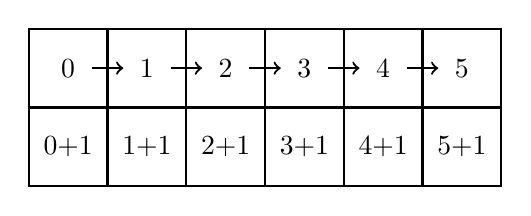
\begin{tikzpicture}
        % Draw the dominoes
        \foreach \x in {0, 1, 2, 3, 4, 5} {
                \draw[thick] (\x, 0) rectangle (\x+1, 2);
                \draw[thick] (\x, 1) -- (\x+1, 1);
            }

        % Label the dominoes
        \foreach \x in {0, 1, 2, 3, 4, 5} {
                \node at (\x+0.5, 1.5) {\x};
                \node at (\x+0.5, 0.5) {\x+1};
            }

        % Draw arrows to show the toppling effect
        \foreach \x in {0, 1, 2, 3, 4} {
                \draw[->, thick] (\x+0.8, 1.5) -- (\x+1.2, 1.5);
            }
    \end{tikzpicture}
\end{center}
Base case $\Leftrightarrow$ we push over domino 0.

Inductive step $\Leftrightarrow$ if domino $m$ topples, then domino $m+1$
topples too.

Inductive hypothesis $\Leftrightarrow$

\begin{remark}The inductive step is usually the hardest part of an inductive argument. However, as the above analogy shows, the base case is essential too: if no domino is pushed over, none will topple!
\end{remark}
\subsection{Examples}
\begin{enumerate}
    \item Prove that

          \[
              1 + 2 + \cdots + n = \frac{n(n+1)}{2}
          \]

          \begin{proof}

              Let $P(n) := 1 + \cdots + n = \frac{n(n+1)}{2}$.

              \textbf{Base case:} When $n = 0$, the LHS = 0 (since the sum is empty) and the RHS = 0 too. So $P(0)$ is true. \\
              \textbf{Inductive Step:} Suppose $P(m)$ is true, i.e.,
              \[
                  1 + \cdots + m = \frac{m(m+1)}{2}
              \]
              Then
              \[
                  \begin{aligned}
                      1 + \cdots + m + (m+1) & = (1 + \cdots + m) + (m+1)                                            \\
                                             & = \frac{m(m+1)}{2} + (m+1) \quad \text{(by our inductive hypothesis)} \\
                                             & = (m+1)\left(\frac{m}{2} + 1\right)                                   \\
                                             & = (m+1)\left(\frac{m+2}{2}\right)                                     \\
                                             & = \frac{(m+1)(m+2)}{2}
                  \end{aligned}
              \]
              So $P(m+1)$ is true too.

              It follows, by induction, that $P(n)$ is true for all $n \in \mathbb{N}$, i.e.,

              \[
                  1 + 2 + \cdots + n = \frac{n(n+1)}{2}
              \]
          \end{proof}
    \item Let $f_n = n^{\text{th}}$ Fibonacci number, defined as the $n^{\text{th}}$ term
          of the sequence defined recursively by:

          \[
              \left\{
              \begin{array}{l}
                  f_0 = 0 \\
                  f_1 = 1 \\
                  f_n = f_{n-1} + f_{n-2} \text{ if } n \geq 2
              \end{array}
              \right.
          \]

        \begin{center}
            \begin{tabular}{|c|c|c|c|c|c|c|c|c|c|}
                \hline
                $n$   & 0 & 1 & 2 & 3 & 4 & 5 & 6 & 7  & 8  \\
                \hline
                $f_n$ & 0 & 1 & 1 & 2 & 3 & 5 & 8 & 13 & 21 \\
                \hline
            \end{tabular}
        \end{center}       
        Now that

          \[
              f_n = \frac{1}{\sqrt{5}} \left[ \left( \frac{1 + \sqrt{5}}{2} \right)^n - \left( \frac{1 - \sqrt{5}}{2} \right)^n \right]
          \]

          Note: $T_{\pm} := \frac{1 \pm \sqrt{5}}{2}$ are the two roots of the quadratic
          equation $x^2 = x + 1$. $T_+$ is known as the golden ratio.

          \begin{proof}

              Let $P(n)$ denote the statement

              \[
                  f_n = \frac{1}{\sqrt{5}} \left( T_+^n - T_-^n \right)
              \]

              We prove that $P(n)$ is true for all $n \in \mathbb{N}$ by induction:

              \textbf{Base case:} $n = 0$:
              \[
                  \begin{aligned}
                      f_0 = 0 & = \frac{1}{\sqrt{5}} \left( T_+^0 - T_-^0 \right)                                                                     \\
                      f_1 = 1 & = \frac{1}{\sqrt{5}} \left( \left( \frac{1 + \sqrt{5}}{2} \right)^1 - \left( \frac{1 - \sqrt{5}}{2} \right)^1 \right) \\
                              & = \frac{1}{\sqrt{5}} \left( T_+^1 - T_-^1 \right)
                  \end{aligned}
              \]
              \\\textbf{Inductive step:} Suppose $P(k)$ is true for all $k < m$. We will prove that $P(m)$ is true too:

              If $m = 0$ or $m = 1$, we verified that $P(m)$ is true in our base case.
              Suppose $m \geq 2$.
              \[
                  \begin{aligned}
                      f_m & = f_{m-1} + f_{m-2} \quad \text{(defining recursion for } f_m\text{)}                                                 \\
                          & = \frac{1}{\sqrt{5}} \left( T_+^{m-1} - T_-^{m-1} \right) \quad \text{(since } P(m-1) \text{ is true, by hypothesis)} \\
                          & + \frac{1}{\sqrt{5}} \left( T_+^{m-2} - T_-^{m-2} \right) \quad \text{(since } P(m-2) \text{ is true, by hypothesis)} \\
                          & = \frac{1}{\sqrt{5}} \left( T_+^{m-1} + T_+^{m-2} \right) - \frac{1}{\sqrt{5}} \left( T_-^{m-1} + T_-^{m-2} \right)   \\
                          & = \frac{1}{\sqrt{5}} \left( T_+^{m-2} (T_+ + 1) \right) - \frac{1}{\sqrt{5}} \left( T_-^{m-2} (T_- + 1) \right)       \\
                          & = \frac{1}{\sqrt{5}} \left( T_+^{m-2} \cdot T_+^2 \right) - \frac{1}{\sqrt{5}} \left( T_-^{m-2} \cdot T_-^2 \right)   \\
                          & = \frac{1}{\sqrt{5}} \left( T_+^m - T_-^m \right)
                  \end{aligned}
              \]

              Thus, $P(m)$ is true too. It follows that $P(n)$ is true for all $n \in
                  \mathbb{N}$, i.e.,

              \[
                  f_n = \frac{1}{\sqrt{5}} \left( T_+^n - T_-^n \right) \text{ for all } n \in \mathbb{N}
              \]
          \end{proof}
          The above proof uses the strong form of mathematical induction.
\end{enumerate}
\begin{theorem} [Principle of Mathematical Induction (strong form)]
    Let $\{P(n)\}_{n \in \mathbb{N}}$ be statements indexed by $n \in \mathbb{N} = \{0, 1, 2, \ldots\}$. Suppose
    \begin{itemize}
        \item (a) $P(0)$ is true
        \item (b) $P(0), P(1), \ldots, P(m) \Rightarrow P(m+1)$ true for all $m \in \mathbb{N}$.
    \end{itemize}

    Then $P(n)$ is true for all $n \in \mathbb{N}$.
\end{theorem}

\begin{proof} Let $Q(n)$ be the statement that

    \[
        P(0), P(1), \ldots, P(n) \text{ are all true.}
    \]

    $Q(0)$ is true $P(0)$ is true.
    Suppose $Q(m)$ is true, i.e.,
    \[
        P(0), \ldots, P(m) \text{ are all true.}
    \]
    By (b) (the strong inductive step), $P(m+1)$ is true.

    Thus, $P(0), \ldots, P(m), P(m+1)$ are all true by (b). It follows that
    $Q(m+1)$ is true too. By induction, $Q(n)$ is true for all $n \in \mathbb{N}$,
    implying that $P(n)$ is true for all $n \in \mathbb{N}$.
\end{proof}

\section{January 22, 2025}
\subsection{Well-Ordering Principle}
\begin{theorem} [Well-ordering principle]
    Let $S \subset \mathbb{N}$ be non-empty. Then $S$ contains a least element $t$, i.e.,
    \begin{itemize}
        \item $t \in S$
        \item $t \leq s$ for all $s \in S$
    \end{itemize}
\end{theorem}

\begin{proof}
    Let $t \in S$. Consider the subset $S' = \{ s \in S : s \leq t \} = S \cap \{0, \ldots, t\}$. Since $S'$ is a non-empty subset of $\{0, \ldots, t\}$, it is finite. Therefore, $S'$ has a least element, say $t'$. By construction, $t' \in S'$ and $t' \leq s$ for all $s \in S'$. Since $S' \subset S$, it follows that $t' \in S$ and $t' \leq s$ for all $s \in S$. Thus, $t'$ is the least element of $S$.
\end{proof}
\begin{corollary}
    $t' \in S$ is a minimal element of $S$.
\end{corollary}

\begin{proof}
    By construction, $t' \in S$ and $t' \leq t$. For any $s \in S$, if $s \leq t$, then $s \in S'$. By the definition of $t'$, we have $t' \leq s$. If $s \notin S'$, then $s > t$, and since $t \geq t'$, it follows that $s > t'$. Therefore, $t' \leq s$ for all $s \in S$.

    This shows that $t'$ is the least element of $S$.

    To prove that every finite subset of $\mathbb{N}$ contains a least element, we
    use mathematical induction. We will show that the well-ordering principle
    implies the strong form of induction.
\end{proof}

\subsection{Connection between the Well-Ordering Principle and Induction}

\begin{theorem}

    Assume the well-ordering principle holds. Then the strong form of induction
    holds too: Suppose $\{P(n)\}_{n \in \mathbb{N}}$ are statements for which:

    \begin{itemize}
        \item[(a)] $P(0)$ is true
        \item[(b)] $P(0), \ldots, P(m-1)$ true $\Rightarrow P(m)$ true for all $m \in \mathbb{N}_{>0}$.
    \end{itemize}

    Then $P(n)$ is true for all $n \in \mathbb{N}$.
\end{theorem}
\begin{proof}
    Let $S = \{ n \in \mathbb{N} : P(n) \text{ is false} \}$. We want to prove that $S$ is empty.

    Suppose $S$ is non-empty. Let $t \in S$ be a least element. Since $P(0)$ is
    true, $0 \notin S$. Therefore, $t \neq 0$, i.e., $t \geq 1$. Since $0, 1,
        \ldots, t-1 < t$, it follows that $0 \notin S, 1 \notin S, \ldots, t-1 \notin
        S$, i.e., $P(0), P(1), \ldots, P(t-1)$ are all true. By assumption (b), it
    follows that $P(t)$ is true, i.e., $t \notin S$. This contradicts $t \in S$.

    It follows that $S$ is empty, i.e., $P(n)$ is true for all $n \in \mathbb{N}$.
\end{proof}
The well-ordering principle perspective often reveals what you should take as
the base case for an inductive argument.
\subsection{Examples}
\begin{enumerate}

    \item

          \[
              \left\{
              \begin{array}{l}
                  F_0 = 0 \\
                  F_1 = 1 \\
                  F_n = F_{n-1} + F_{n-2}
              \end{array}
              \right. \text{ for } n \geq 2.
          \]

          Prove that

          \[
              F_n = \frac{1}{\sqrt{5}} \left( T_+^n - T_-^n \right) \text{ for all } n \in \mathbb{N}.
          \]

          \[
              T_{\pm} = \frac{1 \pm \sqrt{5}}{2}, \text{ the roots of } x^2 = x + 1
          \]

          \begin{proof} Let $S = \{ n \in \mathbb{N} : F_n \neq \frac{1}{\sqrt{5}} \left( T_+^n - T_-^n \right) \}$. We want to prove that $S$ is empty.

              Suppose $S$ is non-empty. Let $t$ be the least element of $S$.

              \begin{itemize}
                  \item Suppose $t \geq 2$. Then
                        \begin{itemize}
                            \item (a) $F_{t-1} = \frac{1}{\sqrt{5}} \left( T_+^{t-1} - T_-^{t-1} \right)$ since $t-1 \in \mathbb{N} \setminus S$
                            \item (b) $F_{t-2} = \frac{1}{\sqrt{5}} \left( T_+^{t-2} - T_-^{t-2} \right)$ since $t-2 \in \mathbb{N} \setminus S$
                        \end{itemize}
                  \item Note: We assume $t \geq 2$ here. Otherwise, $t-1$ and $t-2$ are not both
                        natural numbers.
                        \[
                            \begin{aligned}
                                F_t & = F_{t-1} + F_{t-2} \quad \text{(by the recursive definition of Fibonacci numbers)}                                 \\
                                    & = \frac{1}{\sqrt{5}} \left( T_+^{t-1} + T_+^{t-2} \right) - \frac{1}{\sqrt{5}} \left( T_-^{t-1} + T_-^{t-2} \right) \\
                                    & = \frac{1}{\sqrt{5}} \left( T_+^{t-2} (T_+ + 1) \right) - \frac{1}{\sqrt{5}} \left( T_-^{t-2} (T_- + 1) \right)     \\
                                    & = \frac{1}{\sqrt{5}} \left( T_+^{t-2} \cdot T_+^2 \right) - \frac{1}{\sqrt{5}} \left( T_-^{t-2} \cdot T_-^2 \right) \\
                                    & = \frac{1}{\sqrt{5}} \left( T_+^t - T_-^t \right)
                            \end{aligned}
                        \]
                        Thus, $F_t = \frac{1}{\sqrt{5}} \left( T_+^t - T_-^t \right)$, implying $t
                            \notin S$. This contradicts $t \in S$. It follows that $t = 0$ or $t = 1$.
              \end{itemize}
          \end{proof}
          \begin{remark} Three "leftover cases" form our base case, since our main argument above did not address either of these edge cases.
          \end{remark}
          \begin{itemize}
              \item If $t = 0$,
                    \[
                        F_0 = 0 = \frac{1}{\sqrt{5}} \left( T_+^0 - T_-^0 \right), \text{ so } 0 \notin S
                    \]
              \item If $t = 1$,
                    \[
                        F_1 = 1 = \frac{1}{\sqrt{5}} \left( T_+^1 - T_-^1 \right), \text{ so } 1 \notin S
                    \]
          \end{itemize}

          We've shown:
          \begin{itemize}
              \item If $t \geq 2$, then $t$ cannot be a least element of $S$.
              \item If $t = 0$ or $t = 1$, then $t \notin S$.
          \end{itemize}

          Thus, $S$ contains no least element. This contradicts $S$ being non-empty (by
          the well-ordering principle).

          It follows that $S$ is empty, i.e.,

          \[
              F_n = \frac{1}{\sqrt{5}} \left( T_+^n - T_-^n \right) \text{ for all } n \in \mathbb{N}
          \]

          This perspective is also helpful for rooting out false statements you might try
          to prove by induction.

    \item Let $P(n)$ be the statement:

          \[ P(n) : \text{All collections of } n \text{ boxes are the same color.} \]

          We know, from life experience, this statement is false.

          Let's see why:

          Let $S = \{ n \in \mathbb{N} : P(n) \text{ is false} \}$.

          Suppose $S$ is non-empty. Let $t$ be the least element of $S$. Suppose $t \geq
              3$. Then $P(1)$ and $P(2)$ are true (since $1, 2 \notin S$ by minimality of
          $t$). Let $\{1, \ldots, t\}$ be any collection of $t$ boxes. Divide them into
          two sets

          \[ A = \{1, \ldots, t-1\} \text{ and } B = \{2, \ldots, t\} \]

          Since $t$ is minimal, $P(t-1)$ is true. So all boxes in $A$ are some common
          color, call it $a$. Likewise, all boxes in $B$ are some common color, call it
          $b$. Since $t \geq 3$, the sets $A$ and $B$ overlap. Thus $a = b$. It follows
          that $\{1, 2, \ldots, t\}$ are all the same color, i.e., $P(t)$ is true. Thus
          $t \notin S$, contradicting $t \in S$. Thus, if $t \geq 3$, $t$ cannot be a
          minimal element of $S$.

          For $t = 1$, $P(1)$ is clearly true. So $1 \notin S$. For $t = 2$, $P(2)$ is
          not necessarily true. So at this very last step, our argument breaks down!
\end{enumerate}
\section{January 24, 2025}

\subsection{Arithmetic of \(\mathbb{Z}\)}

We turn from counting properties of \(\mathbb{Z}\) and \(\mathbb{N}\)—these
feature prominently in induction:

\[
    0 \underset{\text{next}}{\rightarrow} 1 \underset{\text{next}}{\rightarrow} 2 \underset{\text{next}}{\rightarrow} 3
\]

to the basic arithmetic operations in \(\mathbb{Z}: +, -, \times\). What about
division??

\begin{definition}
    Let \(a, b \in \mathbb{Z}\). We say that \(b\) divides \(a\) / \(a\) is a multiple of \(b\) / \(a\) is divisible by \(b\) if \(a = bk\) for some \(k \in \mathbb{Z}\). We
    write that as following
    \[ b \mid a\]
\end{definition}

\begin{example}
    The following could be an example:
    \begin{itemize}
        \item Every integer \(b\) divides \(0\).
        \item Every integer is divisible by \(1\).
    \end{itemize}
\end{example}

\begin{fact}
    If \(b \neq 0\), then \(b\) divides \(a\) iff the rational number \(\frac{a}{b}\) is actually an integer.
\end{fact}
\begin{example}
    \[
        \frac{50}{7} = 7.14 \quad \text{(not an integer. So 7 does not divide 50.)}
    \]

\end{example}

\subsection{The Division Algorithm}
\begin{theorem}[Division Algorithm]

    Let \(a, b \in \mathbb{Z}\), \(b \neq 0\). Then there exist
    \begin{itemize}
        \item \(k \in \mathbb{Z}\)
        \item \(r \in \mathbb{Z}\) with \(|r| < |b|\)
    \end{itemize}
    satisfying:

    \[ a = bk + r \]

\end{theorem}

\begin{proof}
    Let \( \frac{a}{b} = k + \alpha \) for some \( k \in \mathbb{Z} \) and \( \alpha \in \mathbb{Q} \) where \( 0 \leq \alpha < 1 \). Multiplying both sides by \( b \), we get:

    \[ a = kb + \alpha b \]

    Define \( r = \alpha b \). Then:

    \[ a = kb + r \]

    Since \( 0 \leq \alpha < 1 \), it follows that \( 0 \leq r < |b| \). Therefore,
    \( r \) is an integer satisfying \( 0 \leq r < |b| \).

    Thus, we have:

    \[ a = kb + r \]

    where \( k \in \mathbb{Z} \) and \( r \in \mathbb{Z} \) with \( 0 \leq r < |b|
    \).

\end{proof}
The result follows.

\begin{remark} In the above proof, we could take \(-\frac{1}{2} \leq \alpha \leq \frac{1}{2}\) (as opposed to \(0 \leq \alpha < 1\)). For \(r = a - kb = b\alpha\),

    \[
        \begin{aligned}
            |r| & = |\alpha b|       \\
                & \leq \frac{|b|}{2}
        \end{aligned}
    \]
\end{remark}
\subsection{Common Divisors}
\begin{definition}
    Let \(a, b \in \mathbb{Z}\). A common divisor \(d\) of \(a\) and \(b\) is an integer \(d \in \mathbb{Z}\) for which:
    \begin{itemize}
        \item \(d \mid a\)
        \item \(d \mid b\)
    \end{itemize}
\end{definition}

\begin{example}
    Let's consider the following examples:
    \begin{itemize}
        \item \(a = \text{anything}, b = 0\)
              \[
                  \left\{
                  \begin{array}{l}
                      \text{common divisors} \\
                      \text{of } a \text{ and } b = 0
                  \end{array}
                  \right\} = \{ \text{divisors of } a \}
              \]

        \item \(a = 26 = 2 \cdot 13\)
              \[
                  \begin{aligned}
                       & b = 65 = 5 \cdot 13 \\
                       & \left\{
                      \begin{array}{l}
                          \text{common divisors} \\
                          \text{of } 26 \text{ and } 65
                      \end{array}
                      \right\} = \{ \pm 1, \pm 13 \}
                  \end{aligned}
              \]

        \item \(a = 91, b = 15\)
              \[
                  \left\{
                  \begin{array}{l}
                      \text{common divisors} \\
                      \text{of } 91 \text{ and } 15
                  \end{array}
                  \right\} = \{ \pm 1 \}
              \]

        \item \(a = 32 = 2 \cdot 2 \cdot 2 \cdot 2 \cdot 2\)
              \[
                  \begin{aligned}
                       & b = 16 = 2 \cdot 2 \cdot 2 \cdot 2 \\
                       & \left\{
                      \begin{array}{l}
                          \text{common divisors} \\
                          \text{of } 32 \text{ and } 16
                      \end{array}
                      \right\} = \{ \pm 1, \pm 2, \pm 4, \pm 8, \pm 16 \}
                  \end{aligned}
              \]
    \end{itemize}

    In all of these examples, observe that there is a common divisor \(d\) of \(a\)
    and \(b\) divisible by all other common divisors.
\end{example}
\begin{definition}
    \(d \in \mathbb{Z}\) is a greatest common divisor of \(a, b \in \mathbb{Z}\) if:
    \begin{enumerate}
        \item \(d\) is a common divisor of \(a\) and \(b\)
        \item if \(e \in \mathbb{Z}\) is a common divisor of \(a\) and \(b\), then \(e \mid
              d\).
    \end{enumerate}
\end{definition}
\begin{lemma}
    Let \(a, b \in \mathbb{Z}\). Let \(e, d\) be greatest common divisors of \(a\) and \(b\). Then \(d = \pm e\).
\end{lemma}

\begin{proof}
    If \(a\) and \(b\) both equal \(0\), then \(0\) is a greatest common divisor of \(a\) and \(b\) and is the only one. If not both \(a\) and \(b\) equal \(0\), then \(e\) and \(d\) are necessarily non-zero (since \(0\) does not divide any non-zero integer).

    Since \(d\) is a greatest common divisor of \(a\) and \(b\), it follows that
    \(d \mid e\). Therefore, there exists some integer \(k \in \mathbb{Z}\) such
    that:
    \[ e = kd \]

    Similarly, since \(e\) is also a greatest common divisor of \(a\) and \(b\), it
    follows that \(e \mid d\). Therefore, there exists some integer \(j \in
    \mathbb{Z}\) such that:
    \[ d = je \]

    Combining these two equations, we get:
    \[ d = je = j(kd) = d \cdot jk \]

    This implies:
    \[ d(1 - jk) = 0 \]

    Since \(d \neq 0\), it follows that:
    \[ 1 - jk = 0 \]

    Hence:
    \[ jk = 1 \]

    This means that \(j\) and \(k\) must be \(\pm 1\). Therefore:
    \[ d = je = \pm e \]

    Thus, \(d\) and \(e\) are equal up to a sign.
\end{proof}
\subsection{Euclidean Algorithm}

\begin{fact} Let $a, b \in \mathbb{Z}$. Then

    \[
        \left\{
        \begin{array}{l}
            \text{common divisors} \\
            \text{of } a \text{ and } b
        \end{array}
        \right\}
        =
        \left\{
        \begin{array}{l}
            \text{common divisors} \\
            \text{of } a - b \text{ and } b
        \end{array}
        \right\}
    \]
\end{fact}
\begin{proof}
    \begin{itemize}
        \item Suppose $d$ is a common divisor of $a$ and $b$. Then $a = jd$ and $b = kd$ for
              some $j, k \in \mathbb{Z}$.
              \[
                  \begin{aligned}
                       & a - b = jd - kd                      \\
                       & = (j - k)d                           \\
                       & \Rightarrow d \text{ divides } a - b
                  \end{aligned}
              \]
              and
              \[
                  b = kd \Rightarrow d \text{ divides } b.
              \]
              Thus, $d$ is a common divisor of $a - b$ and $b$. It follows that
              \[
                  \left\{
                  \begin{array}{l}
                      \text{common divisors} \\
                      \text{of } a \text{ and } b
                  \end{array}
                  \right\}
                  \subset
                  \left\{
                  \begin{array}{l}
                      \text{common divisors} \\
                      \text{of } a - b \text{ and } b
                  \end{array}
                  \right\}
              \]
              Suppose $d$ divides $a - b$ and $b$. Then $a - b = jd$ and $b = kd$ for some
              $j, k \in \mathbb{Z}$.
              \[
                  \begin{aligned}
                       & a = (a - b) + b                  \\
                       & = jd + kd                        \\
                       & \Rightarrow d \text{ divides } a
                  \end{aligned}
              \]
              and
              \[
                  b = kd \Rightarrow d \text{ divides } b.
              \]
        \item Thus, $d$ is a common divisor of $a$ and $b$.
    \end{itemize}
\end{proof}
It follows that
\[
    \left\{
    \begin{array}{l}
        \text{common divisors} \\
        \text{of } a - b \text{ and } b
    \end{array}
    \right\}
    \subset
    \left\{
    \begin{array}{l}
        \text{common divisors} \\
        \text{of } a \text{ and } b
    \end{array}
    \right\}
\]
Combining the latter two containments:
\[
    \left\{
    \begin{array}{l}
        \text{common divisors} \\
        \text{of } a \text{ and } b
    \end{array}
    \right\}
    =
    \left\{
    \begin{array}{l}
        \text{common divisors} \\
        \text{of } a - b \text{ and } b
    \end{array}
    \right\}
\]

More generally, the exact same proof technique may be used to prove:

\[
    \left\{
    \begin{array}{l}
        \text{common divisors} \\
        \text{of } a \text{ and } b
    \end{array}
    \right\}
    =
    \left\{
    \begin{array}{l}
        \text{common divisors} \\
        \text{of } a - kb \text{ and } b
    \end{array}
    \right\}
\]

for every integer $k$.

\subsubsection{Euclidean Algorithm:}

Let $CD(a, b)$ denote the set of common divisors of $a, b \in \mathbb{Z}$.

\textbf{Input:} $(a, b), a, b \in \mathbb{Z}$ with $b \neq 0$ and $|b| \leq |a|$.

\textbf{Output:} A pair $(d, 0)$ with

\[
    CD(a, b) = CD(d, 0)
\]

\textbf{Note:}
\begin{itemize}
    \item Since $d \in CD(d, 0) = CD(a, b)$, $d$ is a common divisor of $a$ and $b$.
    \item If $e \in CD(a, b) = CD(d, 0)$, then $e$ divides $d$ and $e$ divides $0$.
    \item Thus, $d$ is a greatest common divisor of $a$ and $b$.
\end{itemize}

\textbf{The Algorithm:}
\begin{enumerate}
    \item If $b = 0$, return $(a, 0)$.
    \item Otherwise, find $A \in \mathbb{Z}$ for which
          \[
              r = a - Ab \text{ satisfies } |r| < |b|.
          \]
          (By the division algorithm, this is always possible)
    \item Replace $(a, b)$ by $(a^*, b^*) := (b, r)$.
          \begin{itemize}
              \item Go to (1) if $b^* = 0$
              \item Go to the start of step (2) if $b^* \neq 0$
          \end{itemize}
\end{enumerate}

\begin{proposition} The Euclidean algorithm terminates.
\end{proposition}
\begin{proof}Let $(a_n, b_n)$ be the $n^{\text{th}}$ pair calculated in the process of running the Euclidean algorithm. The pair
    \[
        (a_0, b_0), (a_1, b_1), (a_2, b_2), \ldots (a, b)
    \]
    satisfy:
    \begin{itemize}
        \item $|a_m| \geq |b_m|$
        \item $(a_{m+1}, b_{m+1}) = (a_m^*, b_m^*)$
    \end{itemize}

    By construction,

    \[
        |b_m^*| < |b_m|.
    \]

    So $|b_0| > |b_1| > \ldots$ is a strictly decreasing sequence of natural
    numbers. Therefore, the sequence must terminate at by going to step (1) and
    outputting $(a_n, b_n) = (a_n, 0)$ for some (finite) $n \in \mathbb{N}$. This
    proves the algorithm terminates.
\end{proof}
\begin{remark} Given $x, y \in \mathbb{Z}$, we've seen that we can find $A \in \mathbb{Z}$ for which $r = x - Ay$ satisfies $|r| \leq |y|/2$. Applying this choice of $r$ consistently throughout the running of the Euclidean algorithm, Euclidean\_Algorithm$(a, b)$ runs in time $O(\log_2 |b|)$.
\end{remark}
\subsection{Examples}
\begin{enumerate}
    \item Let's find the gcd of 576 and 243.\begin{align*}
              (576, 243) & = (243, 576 - 2 \cdot 243) \\
                         & = (243, 90)                \\
                         & = (90, 243 - 2 \cdot 90)   \\
                         & = (90, 63)                 \\
                         & = (63, 90 - 1 \cdot 63)    \\
                         & = (63, 27)                 \\
                         & = (27, 63 - 2 \cdot 27)    \\
                         & = (27, 9)                  \\
                         & = (9, 27 - 3 \cdot 9)      \\
                         & = (9, 0)
          \end{align*}
          Thereofore,
          \[
              \gcd(576,243) = 9
          \]

    \item Let's find the gcd of 101 and 66.
          \begin{align*}
              (101, 66) & = (66, 101 - 1 \cdot 66) \\
                        & = (66, 35)               \\
                        & = (35, 66 - 1 \cdot 35)  \\
                        & = (35, 31)               \\
                        & = (31, 35 - 1 \cdot 31)  \\
                        & = (31, 4)                \\
                        & = (4, 31 - 7 \cdot 4)    \\
                        & = (4, 3)                 \\
                        & = (3, 4 - 1 \cdot 3)     \\
                        & = (3, 1)                 \\
                        & = (1, 3 - 3 \cdot 1)     \\
                        & = (1, 0)
          \end{align*}
          Thereofore,
          \[
              \gcd(101,66) = 1
          \]

    \item Let's find the gcd of 104 and 80.

          \begin{align*}
              (104, 80) & = (80, 104 - 1 \cdot 80) \\
                        & = (80, 24)               \\
                        & = (24, 80 - 3 \cdot 24)  \\
                        & = (24, 8)                \\
                        & = (8, 24 - 3 \cdot 8)    \\
                        & = (8, 0)
          \end{align*}
          Thereofore,
          \[
              \gcd(104,80) = 8
          \]
\end{enumerate}

We describe an enhanced version of the Euclidean algorithm that allows us to
solve the equation

\[
    x a + y b = d \quad \text{for} \quad x, y \in \mathbb{Z}, \quad d = \operatorname{gcd}(a, b)
\]

\begin{proposition} Let \(a, b \in \mathbb{Z}\). Suppose there are integers \(x, y \in \mathbb{Z}\) for which

    \[
        x \cdot a + y \cdot b = d
    \]

    for some common divisor \(d\) of \(a\) and \(b\). Then \(d\) is a greatest
    common divisor of \(a\) and \(b\).
\end{proposition}
\begin{proof} By assumption, \(d\) is a common divisor of \(a\) and \(b\).

    - Suppose \(e \mid a\) and \(e \mid b\). Then

    \[
        e \mid xa \quad \text{and} \quad e \mid yb \implies e \mid (xa + yb) = d.
    \]

    It follows that \(d\) is a greatest common divisor of \(a\) and \(b\).

\end{proof}
\subsection{The Algorithm}

Let \(a, b \in \mathbb{Z}\) with \(|a| \geq |b|\).

\begin{enumerate}
    \item Form a 3-column table:

          \[
              \begin{array}{c|c|c}
                  d & x & y \\
                  \hline
                    &   &   \\
                    &   &   \\
                    &   &   \\
              \end{array}
          \]

    \item Initialize the first two rows as:

          \[
              \begin{array}{c|c|c}
                  e & x & y \\
                  \hline
                  a & 1 & 0 \\
                  b & 0 & 1 \\
              \end{array}
          \]

    \item Note: \(xa + yb = e\) where \((e, x, y)\) forms a row in this table.

    \item Run the Euclidean algorithm in the left column of the table:

          \[
              \begin{array}{c|c|c}
                  e   & x   & y   \\
                  \hline
                  e'  & x'  & y'  \\
                  e'' & x'' & y'' \\
              \end{array}
          \]

          In particular,

          \[
              \begin{aligned}
                   & e' = x'a + y'b    \\
                   & e'' = x''a + y''b
              \end{aligned}
          \]

          By the division algorithm, we can find \(k \in \mathbb{Z}\) for which \(e''' :=
          e' - k e''\) satisfies \(|e'''| \leq |e''|\).

          Add the new bottom row

          \[
              R''' := R' - k R''
          \]

          to our table:

          \[
              \begin{array}{c|c|c}
                  e    & x    & y    \\
                  \hline
                  e'   & x'   & y'   \\
                  e''  & x''  & y''  \\
                  e''' & x''' & y''' \\
              \end{array}
          \]

          Note that the relation \(x'''a + y'''b = e'''\) holds for the new bottom row of
          our table too, since it holds for the second-to-bottom and third-to-bottom rows
          too:

          \[
              \begin{aligned}
                  x'''a + y'''b & = (x' - kx'')a + (y' - ky'')b                                  \\
                                & = (x'a + y'b) - k(x''a + y''b) \quad \text{(regrouping terms)} \\
                                & = e' - k \cdot e''                                             \\
                                & = e'''
              \end{aligned}
          \]

    \item Stop adding new rows once the bottom two rows become.
\end{enumerate}

The output, i.e., the last two rows \(\Rightarrow\) By the theory of the
Euclidean algorithm (which we've just run in the left (e) - column of our
table),

\[
    d = \operatorname{gcd}(a, b)
\]

Furthermore, since \(xa + yb = e\) for every row \((e, x, y)\) from our table,
it follows that

\[
    x_0 \cdot a + y_0 \cdot b = d
\]

\begin{problem}
Consider the following problems:
\begin{itemize}
    \item Prove that \(\operatorname{gcd}(x_1, y_1) = 1\).
    \item (HARD) Prove that \(a = \pm d \cdot y_1\) and \(b = \mp d \cdot x_1\).
\end{itemize}
\end{problem}
\subsection{Examples}

\begin{enumerate}
    \item Extended Euclidean algorithm for \((596, 243)\):

          \[
              \begin{array}{c|c|c}
                  e   & x  & y  \\
                  \hline
                  596 & 1  & 0  \\
                  243 & 0  & 1  \\
                  90  & 1  & -2 \\
                  63  & -2 & 5  \\
              \end{array}
          \]

    \item Extended Euclidean algorithm for \((3587, 1819)\):

          \[
              \begin{array}{c|c|c}
                  e    & x   & y    \\
                  \hline
                  3587 & 1   & 0    \\
                  1819 & 0   & 1    \\
                  -51  & 1   & -2   \\
                  34   & 35  & -69  \\
                  -17  & 36  & -71  \\
                  0    & 107 & -211 \\
              \end{array}
          \]

          We read off:

          \[
              \begin{aligned}
                   & \left\{
                  \begin{array}{l}
                      -17 = 36 \times 3587 + (-71) \times 1819 \quad \text{(from the next to last row)} \\
                      3587 = 17 \times 211                                                              \\
                      1819 = 17 \times 107
                  \end{array}
                  \right.
              \end{aligned}
          \]
\end{enumerate}

\section{January 31, 2025}

We proved:

\begin{proposition}
    Let $a, b \in \mathbb{Z}$. Let $d = \operatorname{gcd}(a, b)$. There exist integers $x, y \in \mathbb{Z}$ such that
    \[
        xa + yb = d.
    \]
\end{proposition}

Not only did we prove this abstract existence statement, but we saw how to
extract \(x, y\) from the output of the Extended Euclidean Algorithm.

\subsection{Ideals in \(\mathbb{Z}\)}

\(I = \{xayb : x, y \in \mathbb{Z}\} \subset \mathbb{Z}\) is an ideal in the ring \(\mathbb{Z}\) if and only if:

\begin{itemize}
    \item \(I\) is closed under \(+\), \(-\), and \(0 \in I\).
    \item \(r \cdot i \in I\) for all \(i \in I\) and \(r \in \mathbb{Z}\).
\end{itemize}

The above proposition showed that every ideal in \(\mathbb{Z}\) consists of
multiples of a single element. Thus, \(\mathbb{Z}\) is a so-called principal
ideal domain. More on this later.

\subsection{An important application of the above proposition:}

\begin{lemma}
    Let \(a, b \in \mathbb{Z}, n \in \mathbb{Z}\) with \(n \neq 0\). Suppose

    \begin{itemize}
        \item \(n \mid ab\)
        \item \(\operatorname{gcd}(a, n) = 1\).
    \end{itemize}

    Then \(n \mid b\).
\end{lemma}
\begin{proof}
    Since \(\operatorname{gcd}(a, n) = 1\), we can find integers \(x, y\) such that
    \[
        1 = x \cdot a + y \cdot n
    \]

    Multiply both sides of (f) by \(b\):

    \[
        \begin{aligned}
            b & = (x \cdot a + y \cdot n) \cdot b                                                       \\
              & = x \cdot (ab) + (yb) \cdot n \Rightarrow b \text{ is a multiple of } n \text{ by (i)}.
        \end{aligned}
    \]
\end{proof}
\subsection{Application to primes and prime factorization}

\begin{definition} Let \(p \in \mathbb{Z}, p \leq -1\). \(p\) is prime if

    \[
        \{ \text{divisors of } p \} = \{ \pm 1, \pm p \}.
    \]
\end{definition}
\begin{example}

    \begin{itemize}
        \item Prime: \(2, 3, 5, 7, 11, 13, 17, 19, \ldots\)
        \item Not prime: \(4 = 2 \times 2, 6 = 2 \times 3, 9 = 3 \times 3, 91 = 13 \times 7\)
    \end{itemize}
\end{example}
\begin{fact} Non-prime integers are otherwise known as composite.
\end{fact}
\subsection{Sieve of Eratosthenes}

(An algorithm to list all primes in \(\{2, 3, \ldots, N\}\))

\begin{enumerate}
    \item Begin with \(L = \{2, 3, \ldots, N\}, P = \phi\).
    \item Add the smallest element \(s\) of \(L\) to \(P\) and then remove \(s\) and all
          of its multiples from \(L\).
    \item Continue doing this until all elements are removed from \(L\).
\end{enumerate}

\begin{problem} The final \(P\) consists of all prime numbers in \(\{2, \ldots, N\}\). \end{problem}

\subsection{Factorization into primes}

\begin{proposition} Let \(n \in \mathbb{N}\) with \(n \neq 0\). Then \(n\) factors as a product of primes.
\end{proposition}
\begin{proof}
    We prove this by induction on \(n\). \\
    \textbf{Base case:} \(n = 1\). Then \(n = 1\) is the empty product of primes.\\
    \textbf{Inductive step:} Let \(m \geq 2\). Suppose that for \(1 \leq k < m\), \(k\) can be expressed as a product of primes.

    \begin{itemize}
        \item If \(m\) is prime, \(m = m\) expresses \(m\) as a product of 1 prime.
        \item If \(m\) is not prime, \(m = ab\) for some \(1 < a, b < m\).
    \end{itemize}

    Since \(1 \leq a = m / b < m\) and \(1 \leq b = m / a < m\), we can express
    \(a\) and \(b\) as products of primes:

    \[
        \begin{aligned}
             & a = p_1 \ldots p_j \quad p_1, \ldots, p_j \text{ prime} \\
             & b = q_1 \ldots q_t \quad q_1, \ldots, q_t \text{ prime}
        \end{aligned}
    \]

    Then \(m = ab = (p_1 \ldots p_j)(q_1 \ldots q_t)\) expresses \(m\) as a product
    of primes, thus completing the inductive step.

    It follows, by induction, that every integer \(n \geq 1\) can be expressed as a
    product of primes.
\end{proof}
As an application, we can prove the infinitude of primes:

\begin{theorem}
    There are infinitely many primes \(p \in \mathbb{Z}\).
\end{theorem}

\begin{proof}
    Let \(n \in \mathbb{Z}_{>1}\).

    Consider \(n! + 1\), where \(n! = n \times (n-1) \times \cdots \times 2 \times
    1\).

    Since \(n!\) is a product of integers from 1 to \(n\), any prime factor \(p\)
    of \(n! + 1\) must satisfy \(p \mid n! + 1\).

    \textbf{Claim:} \(p > n\).

    Suppose for contradiction that \(p \leq n\).

    Since \(p \leq n\), \(p\) must divide \(n!\). Therefore, \(p \mid n!\).

    But \(p \mid n! + 1\) and \(p \mid n!\) imply \(p \mid (n! + 1) - n! = 1\),
    which is a contradiction since no prime number divides 1.

    Hence, \(p > n\) as claimed.

    Therefore, for every \(n \in \mathbb{Z}_{>1}\), there exists a prime number \(p
    > n\). This implies that there are infinitely many primes.
\end{proof}
\subsection{An important characterization of primes}
\begin{theorem}
    \(p \in \mathbb{Z}\) is prime \(\Leftrightarrow\) for all \(a, b \in \mathbb{Z}\), \(p \mid ab\) implies \(p \mid a\) or \(p \mid b\).
\end{theorem}

\begin{proof}
    \((\Leftarrow)\) Suppose \(p\) is not prime. Then \(p = ab\) for some \(a, b \in \mathbb{Z}\) with \(a, b \neq \pm 1\). Then \(p \mid p = ab\) but \(p \nmid a\) and \(p \nmid b\).

    \((\Rightarrow)\) Suppose \(p\) is prime. Suppose \(p \mid ab\). Note that
    \[
        \left\{
        \begin{array}{l}
            \text{common divisors} \\
            \text{of } a \text{ and } p
        \end{array}
        \right\}
        \subset
        \left\{
        \begin{array}{l}
            \text{divisors of} \\
            p
        \end{array}
        \right\}
        =
        \left\{
        \pm 1, \pm p
        \right\}
    \]
    Since \(\pm p\) are not divisors of \(a\),
    \[
        \left\{
        \begin{array}{l}
            \text{common divisors} \\
            \text{of } a \text{ and } p
        \end{array}
        \right\}
        =
        \left\{
        \pm 1
        \right\}, \text{ i.e., } \operatorname{gcd}(a, p) = \pm 1
    \]
    By our earlier key lemma, since \(p \mid ab\) and \(\operatorname{gcd}(a, p) =
    \pm 1\), it follows that \(p \mid b\).
\end{proof}
\begin{theorem}
    Let \(p \in \mathbb{Z}\) be prime. Let \(a_1, \ldots, a_n \in \mathbb{Z}\) be integers for which \(p \mid a_1 \ldots a_n\). Then \(p \mid a_1\) or \(p \mid a_2 \ldots a_n\).
\end{theorem}

\begin{proof}
    We prove this by induction on \(n\).

    \textbf{Base case:} \(n = 2\). This is the previous case, which states that if \(p \mid a_1 a_2\), then \(p \mid a_1\) or \(p \mid a_2\).

    \textbf{Inductive step:} Suppose the statement is true for some \(n \geq 2\). That is, if \(p \mid a_1 \ldots a_n\), then \(p \mid a_1\) or \(p \mid a_2 \ldots a_n\).

    We need to show that the statement is true for \(n + 1\). Suppose \(p \mid a_1
    a_2 \ldots a_n a_{n+1}\). By the inductive hypothesis, applied to the product
    \(a_1 a_2 \ldots a_n\), we have \(p \mid a_1\) or \(p \mid a_2 \ldots a_n\).
    \begin{itemize}
        \item If \(p \mid a_1\), we are done.
        \item If \(p \mid a_2 \ldots a_n\), then by the base case applied to the product
              \((a_2 \ldots a_n) a_{n+1}\), we have \(p \mid a_2 \ldots a_n\) implies \(p
              \mid a_2\) or \(p \mid a_3 \ldots a_n\).
    \end{itemize}
    Continuing this process, we eventually conclude that \(p \mid a_1\) or \(p \mid a_2\) or \(\ldots\) or \(p \mid a_{n+1}\).

    Therefore, by induction, the statement is true for all \(n \geq 2\).
\end{proof}

We use the latter characterization of primes to prove uniqueness of prime
factorization.
\begin{theorem}
    Every integer \(n \neq 0\) can be written in a unique way as a product of primes.

    More formally, if

    \[
        \begin{aligned}
             & n = p_1^{e_1} \cdots p_k^{e_k} \quad p_1, \ldots, p_k \text{ distinct primes } e_1, \ldots, e_k \in \mathbb{Z}_{\geq 1} \\
             & n = q_1^{f_1} \cdots q_l^{f_l} \quad q_1, \ldots, q_l \text{ distinct primes } f_1, \ldots, f_l \in \mathbb{Z}_{\geq 1}
        \end{aligned}
    \]

    Then \(k = l\) and \((q_1, \ldots, q_l)\) is a rearrangement of \((p_1, \ldots,
    p_k)\), i.e., \(q_i = p_{\sigma(i)}\) for some bijection \(\sigma: \{1, \ldots,
    k\} \rightarrow \{1, \ldots, k\}\) and \(f_j = e_{\sigma(j)}\).
\end{theorem}

\begin{proof}
    We prove this by induction on \(n\).

    \textbf{Base case:} \(n = 1\). \(n = 1\) can only be factored as the empty product over primes. Thus, its factorization into primes is unique.

    \textbf{Inductive step:} Let \(m \geq 2\). Suppose every \(1 \leq k < m\) can be factored uniquely as a product of primes.

    Suppose

    \[
        \begin{aligned}
             & m = p_1^{e_1} \cdots p_k^{e_k} \quad p_1, \ldots, p_k \text{ distinct primes } e_1, \ldots, e_k \in \mathbb{Z}_{\geq 1} \\
             & m = q_1^{f_1} \cdots q_l^{f_l} \quad q_1, \ldots, q_l \text{ distinct primes } f_1, \ldots, f_l \in \mathbb{Z}_{\geq 1}
        \end{aligned}
    \]

    are two factorizations of \(m\). Let \(p = p_1\).

    By (i), \(p \mid m\). By (ii), \(p \mid m = q_1^{f_1} \cdots q_l^{f_l}\). By
    our product characterization of primes, (i) implies \(p \mid q_1\) or
    \(\ldots\) or \(p \mid q_l\).

    Since the \(q\)'s are prime, \(p \mid q_i\) is equivalent to \(p = q_i\).

    Thus, \(p = q_1\) or \(\ldots\) or \(p = q_l\).

    Suppose WLOG that \(p_1 = p = q_1\).

    Then

    \[
        m / p = p_1^{e_1 - 1} p_2^{e_2} \cdots p_k^{e_k} = q_1^{f_1 - 1} q_2^{f_2} \cdots q_l^{f_l}
    \]

    Continuing by the same argument (and letting \(q_1\) play the role of \(p_1\)
    too), we can prove that

    \[
        \begin{aligned}
             & p_1 = p = q_1 \\
             & e_1 = f_1
        \end{aligned}
    \]

    Consider

    \[
        \begin{aligned}
             & m / p^{e_1} = p_2^{e_2} \cdots p_k^{e_k}   \\
             & m / q_1^{f_1} = q_2^{f_2} \cdots q_l^{f_l}
        \end{aligned}
    \]

    By inductive hypothesis (since \(1 \leq m / p^{e_1} < m\)),

    \[
        \begin{aligned}
             & k - 1 = l - 1                                                                                                                                         \\
             & = (q_2, \ldots, q_l) \text{ is a rearrangement of } (p_2, \ldots, p_k) \text{ via a bijection } \sigma: \{2, \ldots, k\} \rightarrow \{2, \ldots, k\} \\
             & q_j = p_{\sigma(j)} \text{ for } j = 2, \ldots, l                                                                                                     \\
             & f_j = e_{\sigma(j)} \text{ for } j = 2, \ldots, k
        \end{aligned}
    \]

    The inductive step follows from this:

    \[
        \begin{aligned}
             & k - 1 = l - 1 \Rightarrow k = l                                                                                                                                   \\
             & = (q_2, \ldots, q_l) \text{ a rearrangement of } (p_2, \ldots, p_k) \text{ via } \sigma: \{2, \ldots, k\} \rightarrow \{2, \ldots, k\}                            \\
             & \Rightarrow (q_1, \ldots, q_l) \text{ is a rearrangement of } (p_1, \ldots, p_k) \text{ via } \tilde{\sigma}: \{1, 2, \ldots, k\} \rightarrow \{1, 2, \ldots, k\} \\
             & \tilde{\sigma}(x) =
            \begin{cases}
                \sigma(x) \text{ if } x \neq 1 \\
                1 \quad \text{if } x = 1
            \end{cases}                                                                                                                                       \\
             & f_j = e_{\sigma(j)} \text{ for } j = 2, \ldots, k                                                                                                                 \\
             & \Rightarrow f_j = e_{\sigma(j)} \text{ for } j = 1, \ldots, k \quad (\text{since } \sigma(1) = 1).
        \end{aligned}
    \]

    By induction, unique factorization in \(\mathbb{Z}\) follows.
\end{proof}
%\section{January 13, 2025}
%\section{January 15, 2025}
%\section{January 17, 2025}
%\section{January 20, 2025}
%\section{January 22, 2025}
%\section{January 24, 2025}
%\section{January 27, 2025}
%\section{January 29, 2025}
%\section{January 31, 2025}

\section{February 3, 2025}
We abstract the properties we need for arithmetic in \(\ZZ\).
\section{February 5, 2025}

\subsection{Examples of Rings}
Last time we we defined abstract rings.
\begin{remark}
    \(1 \in \mathbb{R}\) (ring with \(1\)
\end{remark}

\begin{fact}
    If you take the set of all integers, and you add and multiply them, you get a ring.
\end{fact}

\subsubsection{Non-commutative Rings}
\begin{enumerate}
    \item Let \(V\) be a vector space over \(\mathbb{R}\). The set \(S = \{\text{linear
              transformations } T: V \to V\}\) forms a ring with addition and composition of
          transformations. For \(T, T' \in S\), the addition \(T + T'\) is defined by
          \((T + T')(v) := T(v) + T'(v)\) for all \(v \in V\).
    \item The zero ring is a ring in which the product of any two elements is zero. It
          can be defined as \( R = \{0\} \) with the operations \( 0 + 0 = 0 \) and \( 0
          \cdot 0 = 0 \). This ring has only one element, which is both the additive and
          multiplicative identity.
    \item If \(T, T'\) are both linear transformations from \(V \rightarrow V\). Then \(T \cdot T' = T \cdot T' = \left((T \cdot T)(v)  \right) = T(T'(x))\). That means that the composition of two linear transformations is also a linear transformation. 
\end{enumerate}
\begin{fact}
    If we take two matrices \(T, T'\) and multiply them together \(T \cdot T'\) and \(T' \cdot T\) then they are not the sample. For example
    \[T = \begin{bmatrix}
        0 & 0 \\    
1 & 0
    \end{bmatrix}\] and 
    \[T'=\begin{bmatrix}
        0 & 1 \\
        0 & 0
    \end{bmatrix}\]
    \[T \cdot T' = \begin{bmatrix}
        0 & 1 \\
        0 & 0
    \end{bmatrix}\] and

    \[T' \cdot T = \begin{vmatrix}
    1 & 0 \\
    0 & 0
    \end{vmatrix}\]
    Therefore, we proved that composition of two linear transformations is not commutative.
However, the distributive properties hold.
\end{fact}
%\section{February 7, 2025}
%\section{February 10, 2025}
%\section{February 12, 2025}
%\section{February 14, 2025}
%\section{February 17, 2025}
%\section{February 19, 2025}
%\section{February 21, 2025}
%\section{February 24, 2025}
%\section{February 26, 2025}
%\section{February 28, 2025}
%\section{March 3, 2025}
%\section{March 5, 2025}
%\section{March 7, 2025}
%\section{March 17, 2025}
%\section{March 19, 2025}
%\section{March 21, 2025}
%\section{March 24, 2025}
%\section{March 26, 2025}
%\section{March 28, 2025}
%\section{March 31, 2025}
%\section{April 2, 2025}
%\section{April 4, 2025}
%\section{April 7, 2025}
%\section{April 9, 2025}
%\section{April 11, 2025}
%\section{April 14, 2025}
%\section{April 16, 2025}
%\section{April 18, 2025}
%\section{April 21, 2025}
%\section{April 23, 2025}
%\section{April 25, 2025}
%\section{April 28, 2025}

\end{document}